%%%%%%%%%%%%%%%%%%%%%%%%%%%%%%%%%%%%%%%%%%%
%%%%%%%%%%%%%%%%%%%%%%%%%%%%%%%%%%%%%%%%%%%
%%%%%%%%%%%%%%%%%%%%%%%%%%%%%%%%%%%%%%%%%%%
\chapter{State of the Art}
\label{Sec:star}
In this chapter we will present the state of the art work present in bioinformatical literature with regards to the visualization and analysis of intermolecular interactions of proteins. We will start with overview of existing molecular visualization techniques, then continue with the work related to protein-ligand interactions, where literature covers a substantial amount of diverse research. Then we will continue with analysis of protein-protein interactions. This field is however only sparsely covered in literature.

\section{Molecular Visualization}
styles - cartoon, string, balls and sticks ....
-surfaces
-tools (py mol, analyst)

\section{Detection of Protein Voids}
As we mentioned before, the active site -- the reactive area of the protein is often buried deeply inside of the protein structure and accessible only via protein tunnels. Therefore extraction and analysis of these tunnels is vital for the study of protein-ligand binding. There are several methods for extracting the shape of the protein voids in general, as well as numerous ones focusing on tunnels specifically. The algorithms can be classified into several categories, depending on the approach they use: grid-based, probe-based, surface-based, Voronoi-based, ligand based and path analysis. Most of the algorithms combine several approaches, in order to achieve better results. Moreover, we can differentiate  between algorithms applicable only for static structures and algorithms taking into account molecular dynamics.

Due to the extensiveness of the work related to this topic, we will name only several representatives to demonstrate the basic principles of these approaches. Complete overview of the published tools for detection and analysis of biomolecular cavities can be found in state of the art report by Krone et al. \cite{krone2016visual}.
%In 2012 Berzovsky et. al. published the overview these tools \cite{brezovsky2013software}.

Many algorithms for void detection use a voxel grid to subdivide the 3D space containing the protein. An exaple of a \textbf{grid-based approach} that also utilizes \textbf{path analysis} is the first version of CAVER algorithm \cite{Petrek2006Caver}. Here, each node of the grid is assigned a cost, based on the maximal radius of a hypothetical ball that can be inserted into a node without intersecting voxels occupied by protein atoms -- the larger the radius, the lower the cost. A graph searching algorithm than searches for cheapest path leading from user defined active site to the outer boundary of protein. This path is than taken as tunnel centreline and the detected tunnel is tan represented as a set of maximal spheres placed on centreline.

A slightly dofferent approach is utilized by HOLLOW \cite{Ho2008Hollow} and 3V \cite{voss20103v} algorithms. These algorithms use a combination of \textbf{grid-based} and \textbf{probe-based approach}. Two probe spheres of different sizes are placed in each node of the grid. The probes that do not intersect with protein atoms define the surface of the protein -- large probe defines the outer surface, while the smaller one defines also the inner voids (see Figure \ref{Fig:rollingprobe}). This approach is also referred to as \textit{rolling probe} principle.

Other approaches that utilize voxelized grid and sphere probes include POCKET \cite{levitt1992pocket}, VOIDOO \cite{kleywegt1994detection}, LIGSITE \cite{hendlich1997ligsite}, SURFNET \cite{laskowski1995surfnet}, Roll~\cite{yu2009roll} or dxTuber~\cite{raunest2011dxtuber}.

\begin{figure}[H]
  \centering
  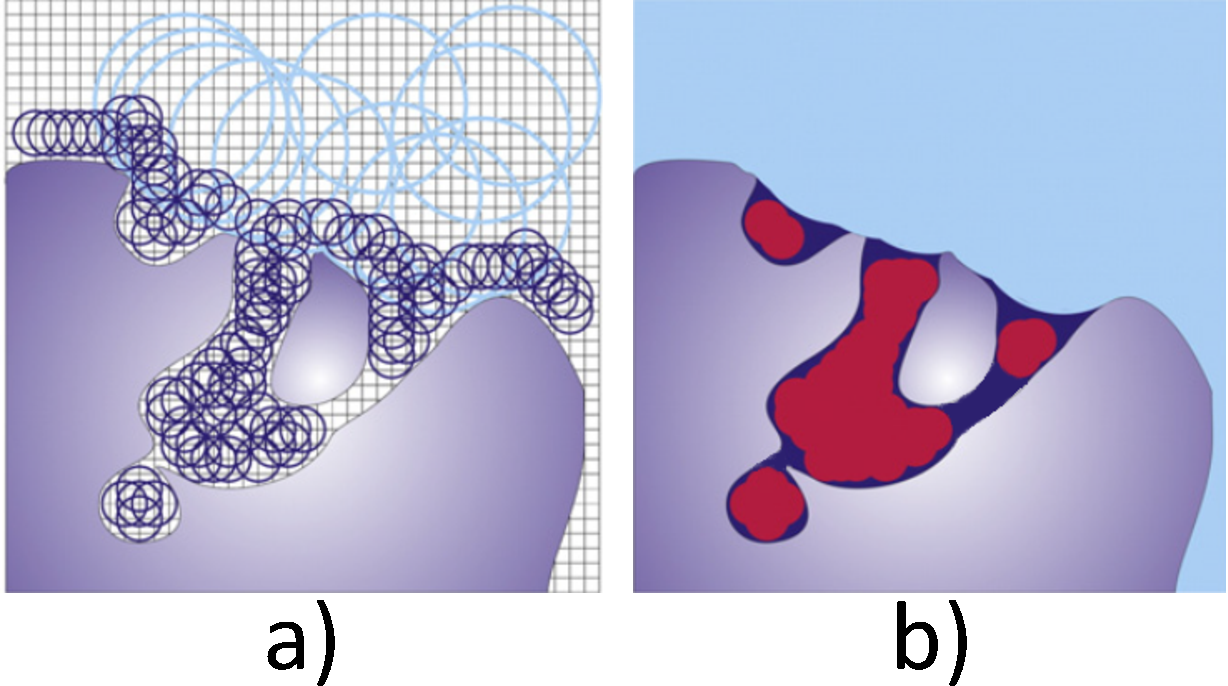
\includegraphics[width=\linewidth]{pictures/rollingprobe.pdf} 
  \caption{a) Rolling probe method. The surface and inner voids of the protein are defined by the placement of probes (large for surrounding and small for voids) in each point of the grid. b) The identified volumes are divided into the protein surrounding (light blue), and internal voids (dark blue), while undetected internal volumes are white. c) HOLLOW represents identified voids using the dummy atoms fitting these voids (red spheres). d) 3V represents detected internal void by voxels (red squares). Image adapted from \cite{brezovsky2013software}.}
  \label{Fig:rollingprobe}  
\end{figure} 

Accuracy of grid-based algorithms strongly depends on the resolution of the voxel grid. At the same time, high resolution of the grid leads to high memory demands of these algorithms. \textbf{Voronoi-based} algorithms in combination with \textbf{path analysis} address these drawbacks by utilizing Voronoi diagrams to subdivide the 3D space of protein structure (see Figure \ref{Fig:voronoi}). Each atom of the protein forms a center of Voronoi cell. The edges are then evaluated by cost function, which assigns the value based on distance of the edge from the cell centres (i.e. atom centres). Then, Dijkstra's algorithm is used on the edge graph to find the best path from the active site towards protein surface. 

\begin{figure}[H]
  \centering
  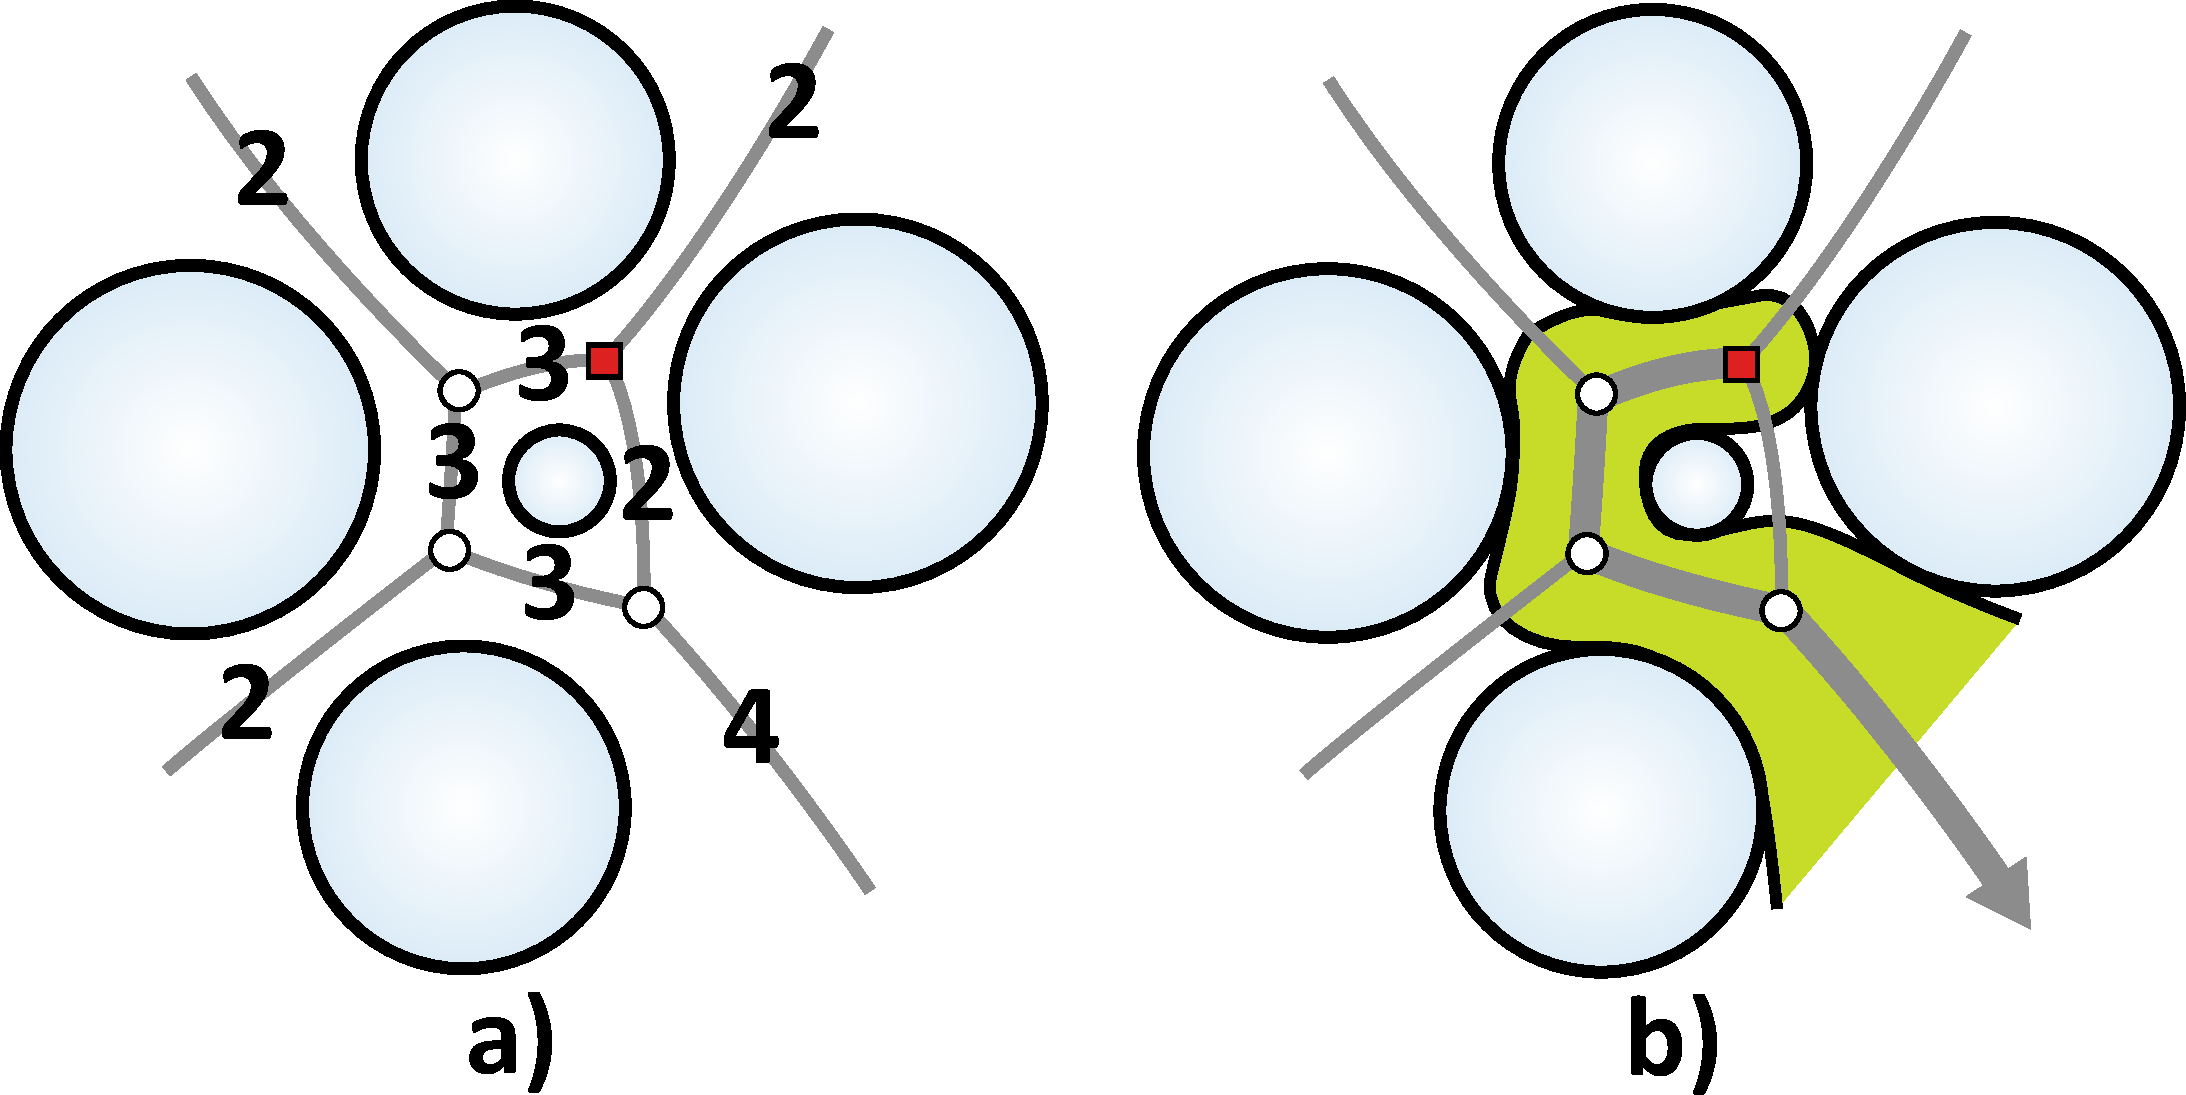
\includegraphics[width=0.7\linewidth]{pictures/voronoi.pdf} 
  \caption{Example of Voronoi-based tunnel detection. a) Evaluated edges. b) Path with highest score found by Dijkstra's algorithm. Red square indicates active site. Image adapted from \cite{caver20}}
  \label{Fig:voronoi}  
\end{figure} 

This principle is used in MOLE~\cite{Petrek2007MOLE} and by Medek et al.~\cite{caver20}. MolAxis \cite{Yaffe2008MolAxis} increases the precision of this algorithm by approximating atom radii, which previous approaches omitted.

While all these approaches offer a solution for static molecules, CAVER 3.0~\cite{caver30} extends them and allows for detection of tunnels taking into account the movement of the protein. It computes tunnel paths for each time frame of MD simulation. Than the corresponding paths are clustered. Thus it is possible to track the evolution of the tunnels in time.

\subsubsection{Path analysis algorithms}
HOLE \cite{Smart1996Hole}
CHUNNEL \cite{Coleman2009CHUNNEL}
POREWALKER \cite{Pellegrini2009PoreWalker}
 




CAST \cite{liang1998anatomy}



\section{Protein-Protein Interactions}
